\subsection{States, Grains and Pillars}
\frame
{
  \frametitle{Top file}
  \begin{itemize}
  \item<1-> Separates environments
  \item<2-> Acts as an overview
  \item<3-> Targets minions
  \item<4-> Defines which states apply
  \end{itemize}
}

\frame
{
  \frametitle{Top file}

  \begin{center}%
    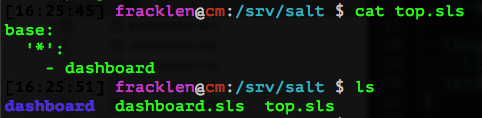
\includegraphics[height=2.5cm]{images/salt_top.png}
  \end{center}%
}

\frame
{
  \frametitle{State file}
  \begin{itemize}
  \item<1-> Defines the content of the state
  \item<2-> References a list of execution modules
  \item<3-> YAML defines name, module and parameters
  \end{itemize}
}

\frame
{
  \frametitle{State file}

  \begin{center}%
    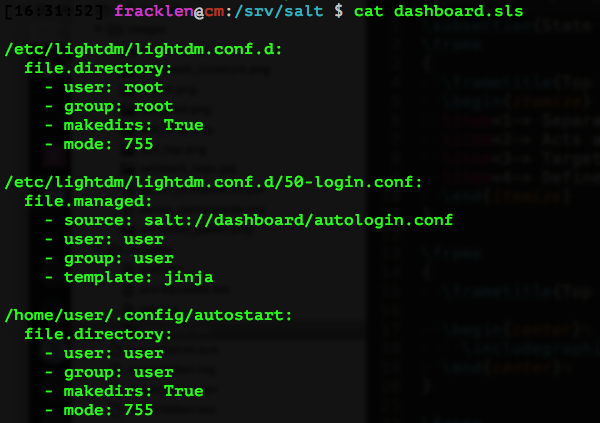
\includegraphics[height=6cm]{images/salt_state.png}
  \end{center}%
}

\frame
{
  \frametitle{Using pillars}
  \begin{itemize}
  \item<1-> Allows use of confidential data in states
  \item<2-> Not searchable
  \item<3-> Not targetable
  \item<4-> Only pushed to the relevant minions
  \end{itemize}
}

\frame
{
  \frametitle{Using pillars}

  \begin{center}%
    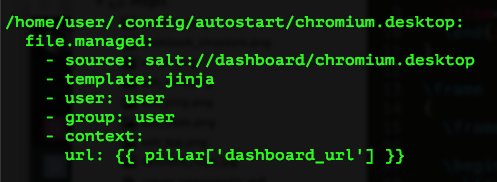
\includegraphics[height=3cm]{images/salt_state_pillar.png}
  \end{center}%

  \begin{center}%
    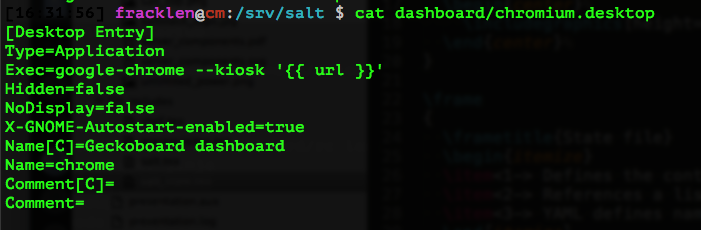
\includegraphics[height=3cm]{images/salt_state_pillar_template.png}
  \end{center}%
}

\frame
{
  \frametitle{Grains vs Pillars}
  \begin{itemize}
  \item<1-> Grains are 'public'
  \item<2-> Pillars are 'private'
  \item<3-> Grains can be targeted
    \begin{itemize}
    \item<4-> salt -G 'os:CentOS' system.reboot
    \item<5-> salt -G 'num\_cpus:32' cmd.run 'some-task'
    \item<6-> salt '*' grains.ls
    \end{itemize}
  \end{itemize}
}

\frame
{
  \frametitle{Defining pillars}

  \begin{center}%
    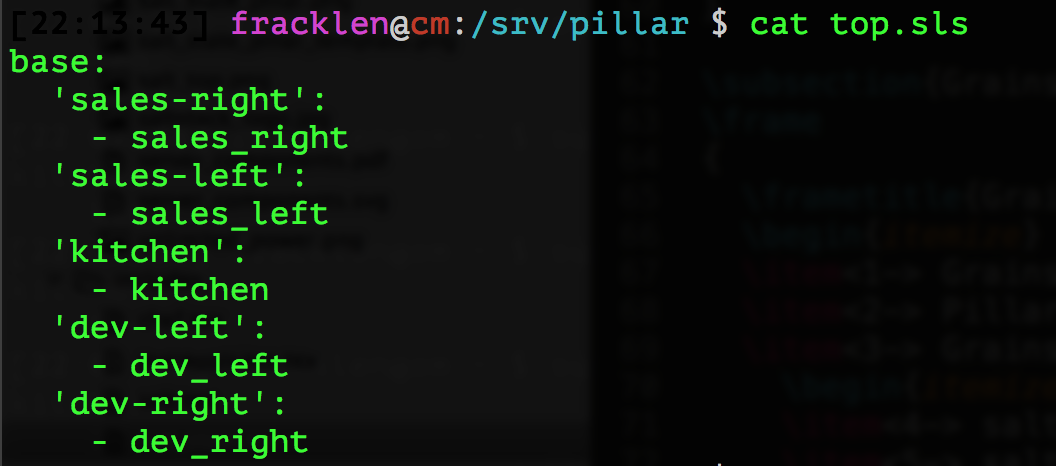
\includegraphics[height=3cm]{images/salt_pillars_top.png}
  \end{center}%
}

\frame
{
  \frametitle{Defining pillars}

  \begin{center}%
    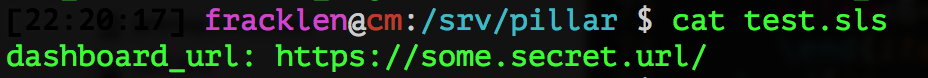
\includegraphics[height=0.8cm]{images/salt_pillars_def.png}
  \end{center}%
}
